\documentclass{article}
\usepackage[utf8]{inputenc}
\usepackage{ graphicx }
\graphicspath{ {img/} }
\usepackage{ geometry}
\geometry{legalpaper, margin=1.3in}
\usepackage{ bbm }
\usepackage{ braket }
\usepackage{ mathrsfs }
\usepackage{ amssymb }
\usepackage{ mathtools }
\usepackage{ amsfonts }
\usepackage{ caption }
\usepackage{ enumitem } % Lists bullet
\usepackage{ tikz }
\usepackage[hidelinks]{ hyperref }

\usetikzlibrary{ quantikz }

\newcommand\eqdef{\mathrel{\overset{\makebox[0pt]{\mbox{\normalfont\tiny\sffamily def}}}{=}}}
\newcommand\eqgoal{\mathrel{\overset{\makebox[0pt]{\mbox{\normalfont\tiny\sffamily goal}}}{=}}}

\title{qk4cs}
\author{}
\date{2021/2022}

\begin{document}

\begin{titlepage}
\begin{center}

\textsc{\LARGE Sorbonne Universite} \\[1cm]
\textsc{\LARGE Master 1 - Quantum Information} \\[1cm]
\textsc{\Large 2021/2022} \\[7cm]


{\huge \bfseries Lecture notes} \\[0.5cm]
{\huge \bfseries -} \\[0.5cm]
{\huge \bfseries Quantum Kinematic} \\[4cm]
\vfill

\includegraphics[scale=0.6]{su.png}
\end{center}
\end{titlepage}

\tableofcontents

\newpage

\section{Introduction}
Physical system which has $d \in \mathbbm{N}$ possible distinguishable states.
Its physical state $\ket{\psi} \in \mathscr{H}$, the Hilbert space $\mathbbm{C}^d$.

\begin{equation}
    \ket{\psi} = \begin{bmatrix} \psi_1\\ \psi_2 \\ \vdots \\ \psi_d\end{bmatrix}
    \text{ and } \forall i, \psi_i \in \mathbbm{C}.
\end{equation}


\noindent
The result of the measurement in the computational basis on
$\ket{\psi}$
 is $i \in [1, \cdots, d]$ with probability $|\psi_i|^2$.
 \\ \noindent
And $\sum_{i=1}^d |\psi_i|^2 = \braket{\psi|\psi} = 1$: the state is normalized.

\subsection{Dirac notation}

\begin{itemize}[label=-]

\item Ket:
\begin{equation}
\ket{\psi} = \begin{bmatrix} \psi_1\\ \vdots \\ \psi_d\end{bmatrix} = \psi_1 \ket{1} + \cdots + \psi_d\ket{d} = \sum_{i=1}^d \psi_i\ket{i}
\end{equation}
\item Bra:
\begin{equation}
\bra{\psi} = \ket{\psi}^\dagger = \ket{\psi^*}^T
\end{equation}
\item Braket:
\begin{equation}
\braket{\psi|\phi}
= \begin{bmatrix} \psi_1^* \cdots \psi_d^*\end{bmatrix} \begin{bmatrix} \phi_1\\ \vdots \\ \phi_d\end{bmatrix}
= \psi_1^*\phi_1 + \cdots + \psi_d^*\phi_d
\end{equation}
$\braket{\psi|\phi} $ is the hermitian product of $\psi$ and $\phi$.
\end{itemize}

\subsection{Measurement in a basis $B$}
$B$ is an orthonormal basis : $B := \{\ket{b_i}\}_{i=1}^d$. B has the following properties:
\begin{equation}
    \begin{aligned}
        \forall i \braket{b_i|b_i} = \delta_{i, j} & \text{ \textit{ (orthonormality)}} \\
        \sum_{i=1}^d\ket{b_i}\bra{b_j} = I & \textit{ (completeness)}
    \end{aligned}
\end{equation}

\begin{figure}[h]
\centering
\begin{quantikz}
    \lstick{$\ket{\psi}$} & \qw & \meter{$B$} & \qw \arrow[r]
    & \rstick{$i$} \qw
\end{quantikz}
\caption{Circuit representation of the measurement of the state $\ket{\psi}$}
\end{figure}

\noindent
The probability of the output of a measurement is given by the following formula :
\begin{equation}
    \mathbbm{P}(out=\ket{b_i}) = |\braket{b_i|\psi}|^2
\end{equation}
The physical object is projected into the state $\ket{b_i}$, this is physically called the "wave packet reduction".

\subsubsection{Qubit}
\begin{equation}
    \ket{0}= \begin{bmatrix} 1 \\ 0 \end{bmatrix}
    \hspace{1.2in}
    \ket{1}= \begin{bmatrix} 0 \\ 1 \end{bmatrix}
\end{equation}
\begin{equation}
    \ket{+} = \frac{1}{\sqrt2}(|0\rangle + |1\rangle)
    \hspace{0.7in}
    \ket{-}= \frac{1}{\sqrt2}(|0\rangle - |1\rangle)
\end{equation}

\subsubsection{Measurement in the basis $\{\ket{\pm}\}$}
\begin{figure}[h]
\centering
\begin{quantikz}
    \lstick{$\ket{0}$} & \qw & \meter{$\pm$} & \qw \arrow[r]
    & \rstick{$
        \begin{cases}
            +, & \text{w.p. $|\braket{+|0}|^2=\frac{1}{2}$}\\
            -, & \text{w.p. $|\braket{-|0}|^2=\frac{1}{2}$}
        \end{cases}$} \qw
\end{quantikz}
\caption{Measure of the state $\ket{0}$ in the basis $\ket{\pm}$}
\end{figure}

\subsection{Wiesner's Quantum Money}
Based on the conjugate coding.

\begin{itemize}
    \item \texttt{bills}:
    \begin{itemize}
        \item serial number
        \item a set of random qubit $E_r \in \{\ket{0}, \ket{1}, \ket{+}, \ket{-}\}^n$
        \item \texttt{mint} knows $\{\text{Serial Number}+\text{Random}\}$, sends it to the bank.
    \end{itemize}
    \item \texttt{Mint}: makes the bill, and gives it to the forger.
    \item \texttt{Forger}: tries to copy the bill, and spends the two to the bank.
    \item \texttt{Bank}: should accept the true one, reject the fake.
\end{itemize}

\begin{table}[h]
    \centering
    \begin{tabular}{c|c|c|c}
    \texttt{mint} & \texttt{forger} basis & \texttt{forger} m. & \texttt{bank} m. \\
    $\ket{0}$ & $\{\ket{0}, \ket{1}\}$ & $\ket{0}$ & $\ket{0} $\\
    $\ket{0}$ & $\{\ket{\pm}\}$ &
    $\begin{cases}
        \ket{+}, & \text{w.p. $\frac{1}{2}$}\\
        \ket{-}, & \text{w.p. $\frac{1}{2}$}
    \end{cases}$ &
    $\begin{cases}
        \ket{0}, & \text{w.p. $\frac{1}{2}$}\\
        \ket{1}, & \text{w.p. $\frac{1}{2}$}
    \end{cases}$
    \end{tabular}
\end{table}

We therefore deduce that
\begin{equation}
\mathbbm{P}(\text{get caugth})= 1-(1-\frac{1}{4})^n = 1-(\frac{1}{4})^n
\end{equation}

\subsection{Bennett and Brassard Quantum Key Exchange: BB84}
Goal: Alice and Bob $\rightarrow$ share a secret bit string , Eve does not know anything.
\\
Settings: Alice and Bob share a quantum channel and an authenticated classical channel.
\\\noindent
Steps:
\begin{enumerate}
    \item Alice prepares $n$ qubits $E_r \in \{\ket{0}, \ket{1}, \ket{+}, \ket{-}\}^n$, and she sends them to Bob
    \item Bob receives . He measures them in the basis $\{B_{0,1}, B_{+,-}\}$
    \item They use the public classical channel to compare the basis Bob used. They throw away the \textit{bad basis} qubits.
    \item Alice and Bob sample the data and compare the error rate $e$. If $e=0$, they keep the key;
        if $e = 25\%$, Eve kowns the key.
\end{enumerate}
What if $0 < e < 25$ ? Eve knows a part of the key.
\section{Unitary transformation}
A transformation is an isolated system, and it is reversible. \\
Let $T$ to be a transformation.
\begin{equation}
    \braket{T(\ket{\psi})|T(\ket{\psi})}=\braket{\psi|\psi}
\end{equation}
$T$ is linear.
\begin{equation}
    T(\alpha\ket{\psi} + \beta\ket{\phi}) = \alpha T(\ket{\psi}) + \beta T(\ket{\phi})
\end{equation}

$T$ acts like an unitary operator.
$T$ corresponds to a complex matrix $U$: $T(\ket{\phi}) = U\ket{\phi}$, $U \in \mathbbm{C}^{n \times n}$,
such that $U^\dagger U= Id$.

In the basis $\{\ket{i}\}_{i=0}^n$,$\braket{T(\ket{\psi})|T(\ket{\psi})} = \braket{i|j} = \delta_{i,j}$
%TODO : add the proof
\\
\\
We have :
\begin{itemize}[label=-]
    \item measurement in computational basis
    \item a machine making arbitrary unitary $U$
\end{itemize}
Let's build a measurement in basis $\{\ket{b_i}\}_i$

\begin{figure}[h]
    \centering
    \begin{quantikz}
        \lstick{$\ket{\psi}$} & \qw & \gate{U} & \phase{U\ket{\psi}}&\meter{} & \qw \arrow[r]
        & \rstick{$i$} \qw
    \end{quantikz}
    \caption{Circuit representation of the measurement unitary exptected behavior}
\end{figure}
\begin{equation}
    \mathbbm{P}(i) \eqdef |\braket{i|U|\psi}|^2 \eqgoal |\braket{b_i|\psi}|^2 \quad \forall \psi
\end{equation}

We want $\bra{i}U=\bra{b_i} \Leftrightarrow U^\dagger\ket{i} = \ket{b_i} \Leftrightarrow U = \sum_i \ket{i}\bra{b_i}$
% TODO : add the proof

Is $U$ an unitary ?

\begin{equation}
    \begin{aligned}
        U^\dagger U &= \Big(\sum_i \ket{b_i}\bra{i}\Big)\Big(\sum_j\ket{j}\bra{b_j}\Big) \\
        &= \sum_{i, j}\ket{b_i}\braket{i|j}\bra{b_j} \\
        &= \sum_i \ket{b_i}\bra{b_i} \\
        &= Id & U \text{ is an unitary. }
    \end{aligned}
\end{equation}

\section{Composition of systems}
Let $A \in \mathscr{H}_A = \mathbbm{C}^{d_A}$ and $B \in \mathscr{H}_B = \mathbbm{C}^{d_B}$
to be two systems in their respective vector spaces.
Then we can construct the space
\begin{equation}
    \mathscr{H}_{AB} = \mathscr{H}_A \otimes \mathscr{H}_B
\end{equation}
Its orthonormal basis is $\{\ket{ij}_{AB}\}_{i, j}$, and
\begin{equation}
    \text{dim}\mathscr{H}_{AB} = \text{dim}\mathscr{H}_A \cdot \text{dim}\mathscr{H}_B
\end{equation}
\\\noindent
If $\ket{\alpha} = \sum_i\alpha_i\ket{i}_A$ and $\ket{\beta} = \sum_i\beta_i\ket{i}_B$,
then
\begin{equation}
    \ket{\phi}_{AB}=\ket{\alpha} \otimes \ket{\beta} = \sum_{i,j}\alpha_i\beta_j\ket{i}_A\ket{j}_B
\end{equation}

and $\ket{\phi}_{AB} \in \mathscr{H}_{AB}$. $\ket{\phi}_{AB}$ is a joint state of systems $A$ and $B$.
\\\noindent
The inner product between two basis states can be defined as
\begin{equation}
    \braket{i,j|k,l}=\braket{i|k}_A\braket{j|l}_B = \delta_{ik}\delta_{jl}
\end{equation}
\\\noindent
The most general state in the space $\mathscr{H}_{AB}$ can be written
\begin{equation}
    \ket{\psi} = \alpha \ket{00} + \beta \ket{01} + \gamma \ket{10} + \delta \ket{11}
\end{equation}
with the usual condition for $\ket{\psi}$ to be normalized:
\begin{equation}
    |\alpha|^2+|\beta|^2+|\gamma|^2+|\delta|^2 = 1
\end{equation}
\\\noindent
Not all states of $\mathscr{H}_{AB}$ are separable into one state of $\mathscr{H}_{A}$ and one state of $\mathscr{H}_{B}$

For example : $\frac{1}{\sqrt{2}}(\ket{00} + \ket{11}) \in \mathscr{H}_{AB}$, but
$\nexists \ket{\alpha}\in \mathscr{H}_A, \ket{\beta}\in \mathscr{H}_B$, such that \\\noindent
$\ket{\alpha}\otimes\ket{\beta} = \frac{1}{\sqrt{2}}(\ket{00} + \ket{11})$.

Necessary condition on the coefficients $(\alpha, \beta, \gamma, \delta)$ of a state to be separable:
\begin{equation}
    \alpha\delta = \beta\gamma
\end{equation}

%TODO : add the part about the partial measurement
\subsection{No cloning theorem}
\subsubsection*{The no cloning theorem}
\begin{equation}
    \text{There is no } U \text{ such that } \forall \ket{\psi} \in \mathscr{H}, U\ket{\psi} = \ket{\psi} \otimes \ket{\psi}
    \in \mathscr{H} \otimes \mathscr{H}.
\end{equation}
\subsubsection*{Proof}
Suppose there exists a such unitary U, then U is a cloning operator.
\begin{equation}
    \begin{aligned}
        U\ket{0} \eqdef \ket{0}\ket{0} \\
        U\ket{1} \eqdef \ket{1}\ket{1}
    \end{aligned}
\end{equation}

By computing the application of $U$ on the state $\ket{+}$, we get on the one hand, by linearity of unitaries
\begin{equation}
    U(\frac{\ket{0}+\ket{1}}{\sqrt{2}}) = \frac{\ket{00}+\ket{11}}{\sqrt{2}}
\end{equation}
\\
and on the other hand, by definition of the operator behavior
\begin{equation}
    U(\frac{\ket{0}+\ket{1}}{\sqrt{2}}) = \frac{\ket{0}+\ket{1}}{\sqrt{2}} \otimes \frac{\ket{0}+\ket{1}}{\sqrt{2}}
    =\frac{1}{2}(\ket{00}+\ket{01}+\ket{10}+\ket{11})
\end{equation}
\\
which is a contradiction. Then such a $U$ operator can not exist.

\subsection{Superdense coding}
\textit{Superdense coding} involves two parties, \texttt{Alice} and \texttt{Bob}.
The protocol allows \texttt{Alice} and \texttt{Bob} to share two bits of information by exchanging just one qubit.
Basically, \texttt{Alice} is in possession of two classical bits of information, which she wishes to send to \texttt{Bob}.

Suppose \texttt{Alice} and \texttt{Bob} initially share a pair of qubits in the entangled state
\begin{equation}
    \ket{\psi} = \frac{\ket{00} + \ket{11}}{\sqrt{2}}
\end{equation}

Here is the procedure.

\begin{table}[h]
    \centering
    \begin{tabular}{c|c|c}
    The state \texttt{Alice} wants to send & The gate she applies & The states after \\
    00 & $I$ & $\frac{\ket{00} + \ket{11}}{\sqrt{2}} = \ket{\phi^+}$  \\
    01 & $Z$ & $\frac{\ket{00} - \ket{11}}{\sqrt{2}} = \ket{\phi^-}$ \\
    10 & $X$ & $\frac{\ket{10} + \ket{01}}{\sqrt{2}} = \ket{\psi^+}$ \\
    11 & $Y$ & $\frac{\ket{01} - \ket{10}}{\sqrt{2}} = \ket{\psi^-}$
    \end{tabular}
\end{table}

\texttt{Alice} send her qubit to \texttt{Bob} and he measures the resulting pair in the base \\
$\{\ket{\phi^+}, \ket{\phi^-},\ket{\psi^+}, \ket{\psi^-}\}$. This is indeed a basis, and its name is the \textit{Bell basis},
and the states are called the \textit{Bell states}.


\subsection{Quantum teleportation}


\section{Measurements}
\subsection{Projective measurement}
A projective measurement is described by an observable, a Hermitian operator. They are defined by a set of projectors $\{\Pi_j\}_{j=1}^k, k \leq d$.\\
Projectors properties:
\begin{equation}
    \forall j, \Pi_j^2 = \Pi_j \qquad \Pi_j\Pi_i = \delta_{i,j}\Pi_j
\end{equation}
\\\noindent
A projector is defined as follows:
\begin{equation}
    \Pi_j = \sum_{l=1}^{d_j}\ket{l_l^j}\bra{l_l^j}
\end{equation}
Upon measuring the state $\ket{\psi}$, the probability of getting result $j$ is given by
\begin{equation}
    \braket{\psi|\Pi_j|\psi} = \| \Pi_j\ket{\psi}\|^2
\end{equation}
Given that outcome $j$ occured, the state of the quantum system immediately after the measurement is
\begin{equation}
    \frac{\Pi_j\ket{\psi}}{\| \Pi_j\ket{\psi}\|^2}
\end{equation}

\subsection{Observables}
Observables correspond to physical quantities, with values in $\mathbbm{R}$.
They are well defined in a basis $\{\ket{b_i}\}_i$ (i.e $\forall \ket{b_i}, \exists a_i \in \mathbbm{R})$

\paragraph{Note :} $\alpha\ket{b_1} + \beta\ket{b_2}$ has \textbf{not always} a well defined value.

An observable is defined as follow:
\begin{equation}
    O \eqdef \sum_i o_i \underbrace{\ket{b_i}\bra{b_i}}_{\text{projector on $\ket{b_i}$}}
    = \sum_j o_j \Pi_j
\end{equation}
$O$ is diagonalizable by definition and $O^\dagger = O$: $O$ is hermitian.
$$
\text{Shape of $O$ } :
\begin{pmatrix}
    o_1 & 0 & \cdots & 0 \\
    0 & o_2 & \cdots & \vdots \\
    \vdots  & \vdots  & \ddots & \vdots  \\
    0 & \cdots & \cdots & a_d
\end{pmatrix}
$$

The probability of getting the result $i$ by measuring $O$ on a state $\ket{\psi}$ is $\braket{\psi|\Pi_i|\psi}$
\subsubsection{Expectation value and standard deviation}

The expectation value of $O$, written $\langle O\rangle$, is given by
\begin{equation}
    \begin{aligned}
        \langle O\rangle
            & = \sum_i o_i \mathbbm{P}(i\ket{\psi}) \\
            & = \sum_i o_i \|\Pi_i\ket{\psi}\|^2 \\
            & = \sum_i o_i \braket{\psi|\Pi_i|\psi} \\
            & = \bra{\psi}\sum_i o_i \Pi_i \ket{\psi} \\
            & = \braket{\psi | O |\psi}
    \end{aligned}
\end{equation}

From this formula for the expectation value follows a formula for the standard deviation associated to the observation of $O$
\begin{equation}
    \Delta^2 O = \langle(O - \langle O \rangle)^2\rangle = \langle O^2 \rangle - \langle O \rangle^2
\end{equation}

\paragraph{Note:} If $\ket{\psi}$ is an eigenstate of $O$, then $O\ket{\psi} = \lambda \ket{\psi}$.
\\
Hence:
\begin{equation}
    \begin{aligned}
        \braket{O}
            & = \braket{\psi | O | \psi} \\
            & = \braket{\psi | \lambda | \psi} \\
            & = \lambda\braket{\psi|\psi } \\
            & = \lambda
    \end{aligned}
\end{equation}
\\
And:
\begin{equation}
    \begin{aligned}
        O\ket{\psi} = \braket{O} \ket{\psi}
            & \Rightarrow \Delta^2 O = (\lambda^2 - \lambda^2) = 0 \\
            & \Rightarrow \Delta O = 0
    \end{aligned}
\end{equation}

\subsubsection{Commutators}
A key property of quantum physics is the existence of incompatible measurements:
for any physical property $A$, there exists another physical property $B$ which is incompatible
with $A$. The incompatible means it is physically impossible to prepare a state $\ket{\psi}$
which gives perfectly predictible outputs for both measurements $A$ and $B$.
Let us first assume $A$ and $B$ to be observables.
A key property of this pair of observable is their commutator
\begin{equation}
    [A,B]:= AB-BA
\end{equation}

If $A$ and $B$ commute (i.e $[A,B]=0 \Leftrightarrow AB = BA$), there exists a basis
such that the result of a measurement of $A$ and a measurement of $B$ are perfectly defined.

Conversely, if such a basis exists, then $[A,B]=0$

Therefore, if $A$ and $B$ do not commute, they correspond to incompatible measurements.
(The proofs are in the $4^{th}$ tutorial.)

\subsubsection{The Robertson-Heisenberg uncertainty relation}
This relation evaluates the sharpness of two observables we will call $A$ and $B$ through
the standard deviations $\Delta A$ and $\Delta B$, and the states that, for any state $\ket{\psi}$
and any observable $A$ and $B$

\begin{equation}
    \Delta A \Delta B \geq \frac{1}{2}|\braket{\psi|[A,B]|\psi}
\end{equation}

\subsubsection{Anti-commutator}
The anti commutator of two observables $A$ and $B$ is defined by
\begin{equation}
    \{A,B\} = AB+BA
\end{equation}

\subsubsection*{Example}
Using the Pauli matrix $\sigma_x = X =
    \begin{bmatrix}
    0 & 1 \\
    1 & 0
    \end{bmatrix}
    = \ket{+}\bra{+} - \ket{-}\bra{-}
    $.
\\\noindent
Known results : $X\ket{+} = \ket{+}$ and $X\ket{-}=-\ket{-}$.
\\\noindent
We define $\ket{\theta}:=\cos\theta\ket{0}+\sin\theta\ket{1}$
\\\noindent
Then
\begin{equation}
    \begin{aligned}
        \langle X \rangle_{\ket{\theta}}
            & = \braket{\theta | X |\theta} \\
            & = [\cos \theta \sin \theta]
                \begin{bmatrix}0 & 1 \\ 1 & 0 \end{bmatrix}
                \begin{bmatrix} \cos \theta\\ sin \theta \end{bmatrix} \\
            & = 2 \sin\theta\cos\theta \\
            & = sin 2\theta
    \end{aligned}
\end{equation}


\subsection{Generalized measurements}
A generalized measurement is defined by
\begin{equation}
    \{K_i\}_i \text{ such that } \sum_i K_i^\dagger K_i=Id
\end{equation}
where the $K_i$ are called Kraus Operators.
The probability of getting the result $i$ from a general measurement operator is given by
$\mathbbm{P}(i) = \|K_i\ket{\psi}\|^2$
, and the state of the system just after the measurement is $K_i\ket{\psi}=\frac{K_i\ket{\psi}}{\|K_i\ket{\psi}\|^2}$

\subsubsection*{Generalized measurement $\rightarrow$ Operator}
If $i \in \{1\}$ then
$K_1^\dagger K_1=Id \Rightarrow K_1$ is unitary.%FIXME: not sure of that.

\subsubsection*{Generalized measurement $\rightarrow$ Set of projectors}
If $K_i := \Pi_i$ then $\sum_i K_i^\dagger K_i = \sum_i \Pi_i^\dagger\Pi_i = \sum_i \Pi_i = Id$

\subsubsection*{Example}
With prob. $P_j$, I measure $\{\Pi_{ij}\}_i \text{ } (\sum_i \Pi_{ij} = Id)$ and I measure $U_j$ on the output state.
%TODO : add the scheme
Probability of getting $ij$ :
\begin{equation}
    \begin{aligned}
        \mathbbm{P}(ij)
            &= P_j\braket{\psi | \Pi_{ij} U^\dagger U \Pi_{ij} | \psi} \\
            &= P_j\braket{\psi|\Pi_{ij}|\psi}
    \end{aligned}
\end{equation}
\noindent
And the resulting state is $\dfrac{U\Pi_{ij}\ket{\psi}}{\|\Pi_{ij}\ket{\psi}\|^2}$

\noindent
Let $\{K_{ij} =\sqrt{P_j} U \Pi_{ij}\}_{ij}$, then
\begin{equation}
    \begin{aligned}
        \sum_{ij} K_{ij}^\dagger K_{ij}
            & = \sum_{ij} P_j \Pi_{ij} U^\dagger U \Pi_{ij} \\
            & = \sum_j P_j \sum_i \Pi_{ij} \\
            & = \sum_j P_j \\
            & = Id
    \end{aligned}
\end{equation}
\noindent
Can we associate each set $\{K_i\}_i$ with a $U$ and a $\{\Pi_i\}_i$ ?
\begin{figure}[h]
    \centering
\begin{quantikz}
        \lstick{$\ket{\psi}_I$}
        & \qw \gategroup[2,steps=5,style={dashed,rounded corners,fill=blue!20, inner xsep=2pt},background]{{\sc $\{K_i\}_i$}}
        & \qw
        & \qw
        & \gate[2]{U}
        & \qw\arrow[r]
        &
        & \text{ouput $o$}
        \\
        &
        &
        & \lstick{   $\ket{0}_A$}
        & \qw
        & \meter{M$\{\ket{i}\}$}
        & \qw \arrow[r]
        & \text{ }i
    \end{quantikz}
    \caption{Circuit representation of such $U$ and $\{\Pi_i\}_i$. \\Note : $\mathscr{H}_A\otimes \mathscr{H}_I = \mathscr{H}_O\otimes\mathscr{H}_M$}
\end{figure}
\\\noindent
$\forall i,$ the output state of the system is
\begin{equation}
    \label{output-state-kraus}
    (I_o \otimes \ket{i}_M\bra{i})U\ket{\psi}\otimes\ket{0}_A = \ket{i}_M\braket{i|U|0}_A\ket{\psi}_I
\end{equation}
Assume $K_i = _M\braket{i|U|0}_A$. With (\ref{output-state-kraus}), we deduce that the output state is
$K_i\ket{\psi}$, w.p. $\braket{\psi|K_i^\dagger K_i|\psi}$.
Is $\{K_i\}_i$ a valid set of operators ?
\begin{equation}
    \begin{aligned}
        \sum_i K_i^\dagger K_i
        & = \sum_i (_A\bra{0}\otimes I_I) U^\dagger (\ket{i}_M \otimes I_O)(I_O \otimes _M\bra{i})U(I_I\otimes \ket{0}_A)\\
        & = (_A\bra{0}\otimes I_I)
        \underbrace{U^\dagger (
        \underbrace{
            \underbrace{
                \sum_i \ket{i}_M}_{=I_M}
                    \otimes I_O
            }_{=I_{OM}})
            (I_O \otimes _M\bra{i})
        }_{= I_{OA}}(I_I\otimes \ket{0}_A) \\
        & = (_A\bra{0}\otimes I_I)I_{OA}(I_I\otimes \ket{0}_A) \\
        & = I_O \qquad \text{$\{K_i\}_i$ is a valid set.}
    \end{aligned}
\end{equation}

\subsubsection*{$\{K_i\}_i \rightarrow$ Unitary}
Let $U := \sum_i K_i \otimes \ket{i}_{MA}\bra{0} + \cdots $.
The $\cdots$ represents extra terms used to make $U$ a unitary, but can be neglected in the computation.
By tensoring with $\ket{0}_A$, we obtain
\begin{equation}
    U\ket{\psi}\otimes \ket{0}_A = \sum_i K_i \ket{\psi}\otimes\ket{i}
\end{equation}
And then
\begin{equation}
    \begin{aligned}
        _A\braket{0 |U^\dagger U|0}_A
            & = _A\bra{0}(\sum_i\ket{0}_{AM}\bra{i} K_i^\dagger \cdot \sum_j K_j\ket{j}_{AM}\bra{0})\ket{0}_A \\
            & = \underbrace{_A\braket{0|0}_A}_{=1} \cdot \sum_{ij}(_M\bra{i}\otimes K_i^\dagger)(\ket{j}_M\otimes K_j) \underbrace{_A\braket{0|0}_A}_{=1} \\
            & = \sum_{ij}\underbrace{\braket{i|j}}_{\delta_{ij}} K_i^\dagger K_j \\
            & = \sum_i K_i^\dagger K_i \\
            & = Id
    \end{aligned}
\end{equation}
\subsection{POVMs}
POVMs means Projective Operator Valued Measure :
we "only care about the output $i$, not the state $K_i\ket{\psi}$".
The probability of getting $i$ is $\braket{\psi | K_i^\dagger K_i | \psi}$.\\
Let $E_i = K_i^\dagger K_i$.
POVMs are then defined by the set $\{E_i\}_i$, such that $\sum_i E_i = Id, E_i\geq 0$.\\

$E_i$ is semi-definite positive: $ \forall \psi, \braket{\psi|E_i|\psi} \geq 0$. This implies that $E_i$ is hermitian, and all its eigenvalues are $\geq 0$.
\subsubsection*{POVM $\rightarrow$ Kraus operators}
Let $K_i = \sqrt{E_i}$. $\{K_i\}_i$ is a well defined set of operators.

\subsection{The global phase}
\paragraph{Lemma: }
The global phase is irrelevant\\
Of couse, the state $\ket{\psi} \neq e^{i\phi}\ket{\psi}$

\paragraph{Proof: }
First, we have
\begin{equation}
    |\braket{\psi|e^{i\phi}|\psi}|^2 = |e^{i\phi}|^2 = 1
\end{equation}

Using the generalized measurements $\{K_i\}_i$ such that $\sum_i K_i = Id$
\\\noindent
Then:
\begin{equation}
    K_ie^{i\phi}\ket{\psi} = e^{i\phi}K_i\ket{\psi}
\end{equation}
\noindent
The phase of the input is the same as the phase of the output.
\\\noindent
And
\begin{equation}
    \begin{aligned}
        \|K_ie^{i\phi}\ket{\psi}\|^2_2
            & =\begin{cases}
               \| K_i \ket{\psi} \|_2^2 = & \sqrt{ \mathbb{P}(i\ket{\psi})} \\
               \|e^{i\phi} K_i\ket{\psi}\|_2^2 & \sqrt{\mathbb{P}(i|e^{i\phi}\ket{\psi})}
            \end{cases}
    \end{aligned}
\end{equation}
\\\noindent
Hence, the global phase is irrelevant, and there is no way to measure the global phase.
\\\noindent
However, the relative phase is important for later computations.
\begin{equation}
    \frac{1}{\sqrt{2}}(\ket{0}+\underbrace{e^{i\phi}}_{\text{relative phase}}\ket{1})
\end{equation}

\subsection{General quantum state}
\subsubsection*{Number of parameters to describe a quantum state}
Let $\mathscr{H} = \mathbbm{C^d}$ and $\ket{\psi} \in \mathscr{H}: \ket{\psi} = \sum_{i=0}^d \alpha_i \ket{i}$
, (with $\alpha_i \in \mathbbm{C}$ and $\sum_i |\alpha_i|^2=1$). If we consider $\alpha_i \in \mathbbm{R}$
is the global phase, then $2d-2$ real parameters are needed to represent the quantum state.

\subsubsection*{Example}
Qubit in $\mathscr{H}$:
\begin{itemize}[label=-]
    \item $d=2 \rightarrow 2\cdot2-2 = 2$ right parameters : $(\theta, \varphi)$.
    \item $d=3 \rightarrow 4$ real parameters.
\end{itemize}
A quantum state can be written, with the parameters $\theta$ and $\varphi$ as
\begin{equation}
    \ket{\theta, \varphi} = \cos \frac{\theta}{2}\ket{0} + e^{i\varphi}\sin \frac{\theta}{2}\ket{1}
\end{equation}

\section{Bloch sphere}
\begin{figure}[h]
    \centering
    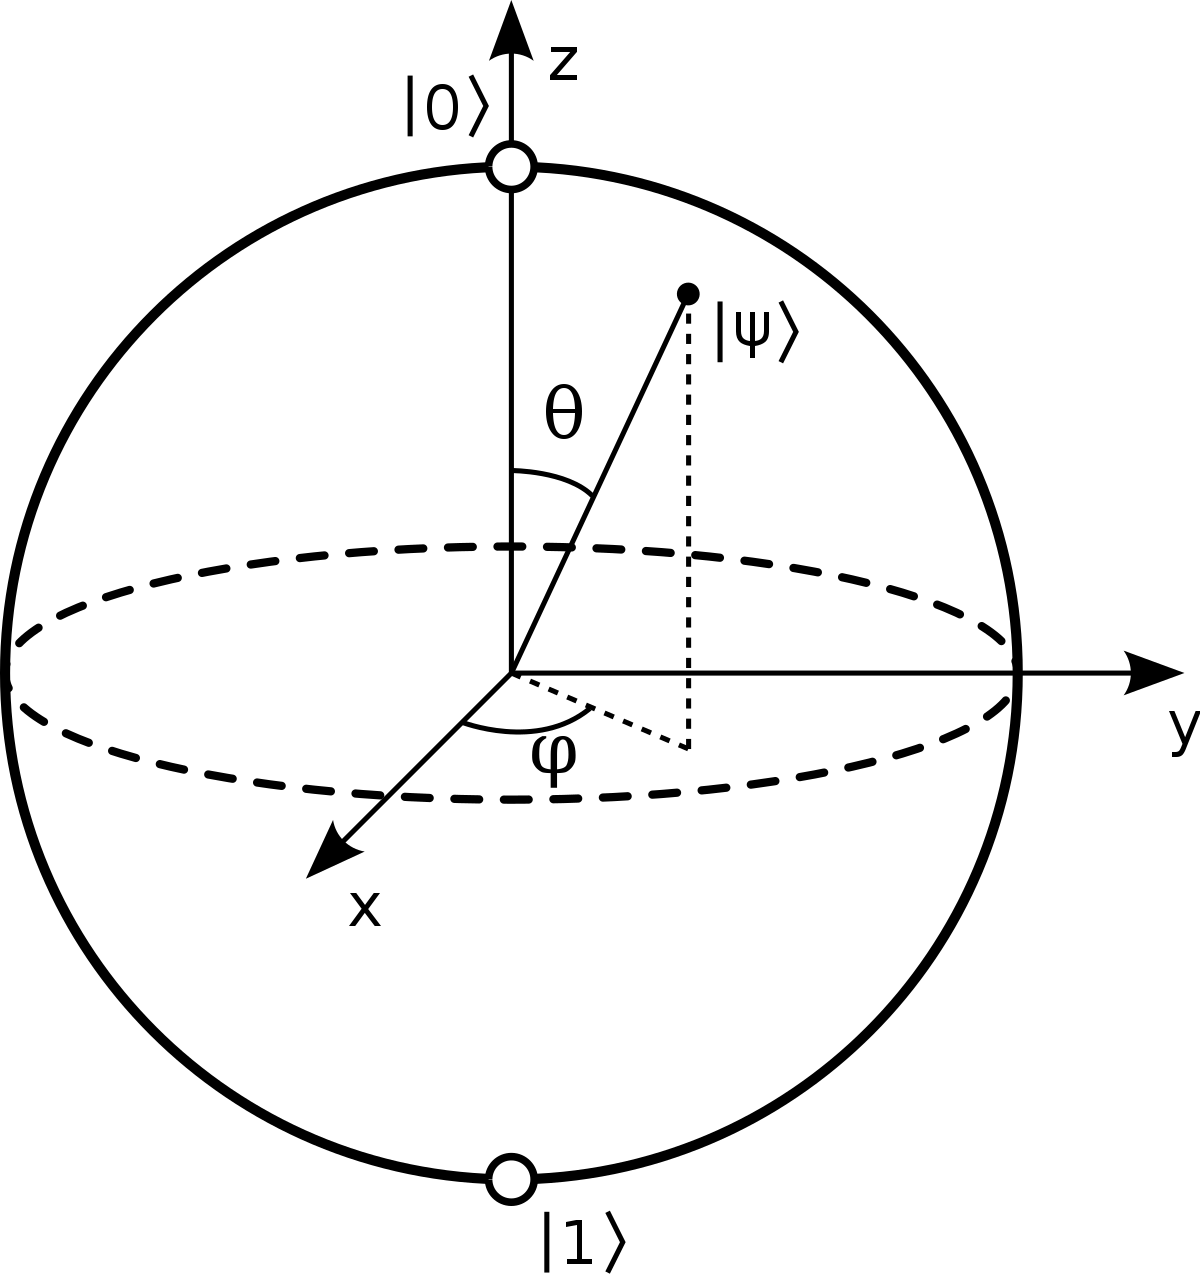
\includegraphics[scale=0.15]{bloch-sphere.png}
    \caption{Graphical representation of a quantum state in the Bloch sphere}
\end{figure}

We will denote $\ket{\psi}$ as the vector $\vec{m}$ in the later computations.
\begin{equation}
    \begin{aligned}
        \vec{m} & = \begin{bmatrix}
            u \\ v \\ w
        \end{bmatrix} \text{such that } u^2 + v^2 + w^2 = 1 \\
        \vec{m} & =
        \begin{bmatrix}
            \label{def-vect-m}
            \cos \theta \cdot \cos \varphi \\
            \sin \theta \cdot \sin \varphi \\
            \cos \theta &
        \end{bmatrix}
    \end{aligned}
\end{equation}

Are $\vec{m}$ and $\vec{-m}$ orthogonal ?
\begin{equation}
    \label{m-m-orthogonal}
    \begin{aligned} % le bordel
        \braket{m|-m}
            & = \braket{\theta,\varphi|\pi-\theta,\varphi+\pi[2\pi]} \\
            & = \Big(\cos\frac{\theta}{2}\bra{0}+e^{i\varphi}\sin\frac{\theta}{2}\bra{1}\Big)
                \Big(\underbrace{\cos(\frac{\pi}{2}-\frac{\theta}{2})}_{\sin\frac{\theta}{2}}\ket{0}+e^{i(\varphi+\pi)}
                \underbrace{\sin(\frac{\pi}{2}-\frac{\theta}{2})}_{\cos\frac{\theta}{2}}\ket{1}\Big) \\
            & = \cos\frac{\theta}{2}\sin\frac{\theta}{2}\braket{0|0}
                +e^{i\varphi}\sin\frac{\theta}{2}(-e^{i\varphi})\cos\frac{\theta}{2}\braket{1|1} \\
        \braket{m|-m}
            & = 0
    \end{aligned}
\end{equation}

Orthogonal states in the Hilbert space correspond to opposite vectors in the Bloch sphere.

\section{Pauli operators}
\subsection{Pauli matrices and properties}
There are four extremely useful two by two matrices called the \textit{Pauli matrices}.
$$
\begin{aligned}
    \sigma_0 \equiv I \equiv &
        \begin{bmatrix}
            1 & 0 \\ 0 & 1
        \end{bmatrix}
    \quad & \quad
    \sigma_1 \equiv \sigma_x = X \equiv &
        \begin{bmatrix}
            0 & 1 \\ 1 & 0
        \end{bmatrix}
    \\
    \sigma_2 \equiv \sigma_y \equiv Y \equiv &
        \begin{bmatrix}
            0 & -i \\ i & 0
        \end{bmatrix}
    \quad & \quad
    \sigma_3 \equiv \sigma_z \equiv Z \equiv &
        \begin{bmatrix}
            1 & 0 \\ 0 & -1
        \end{bmatrix}
\end{aligned}
$$
\subsubsection*{Properties}
\begin{itemize}[label=-]
    \item they are indeed hermitian:
    \begin{equation}
        \forall i \in \{1, 2, 3\} f\quad \sigma_i^\dagger\sigma = \sigma_i^2 = Id
    \end{equation}
    \item braket decomposition
    \begin{equation}
        \begin{aligned}
            \sigma_x & = \ket{0}\bra{1} + \ket{1}\bra{0}
            \\
            \sigma_y & = -i\ket{0}\bra{1} + i\ket{1}\bra{0}
            \\
            \sigma_z & = \ket{0}\bra{1} - \ket{1}\bra{1}
        \end{aligned}
    \end{equation}
    \item commutation relation % may put this in the commutator section
        \begin{equation}
            [X,Y] = 2iZ; \quad [Y, Z] = 2iX; \quad [Z,X] = 2iY
        \end{equation}
\end{itemize}

\subsubsection{Expectation values of the operators}
\begin{itemize}[label=-]
    \item measure $\sigma_z$ on the state $\ket{\theta, \varphi}$
    \begin{equation}
        \begin{aligned}
            \braket{\sigma_z}
                & = \braket{\theta, \varphi|Z|\theta, \varphi} \\
                & = \frac{1}{2} + \frac{1}{2}\cos\theta - \frac{1}{2} + \cos\theta \\
                & = \cos \theta = w \text{  (the $w$ component of $\vec{m}$)}
        \end{aligned}
    \end{equation}
    \item measure $\sigma_x$ on the state $\ket{\theta, \varphi}$
    \begin{equation}
        \begin{aligned}
            \braket{\sigma_x}
                & = \braket{\theta, \varphi|X|\theta, \varphi} \\
                & = \Big(\cos\frac{\theta}{2}\bra{0}+e^{i\varphi}\sin\frac{\theta}{2}\bra{1}\Big)
                    + \underbrace{\Big(\cos\frac{\theta}{2}\ket{1}+e^{i\varphi}\sin\frac{\theta}{2}\ket{0}\Big)}_{=X\ket{\theta, \varphi}} \\
                & = \cos\frac{\theta}{2}\sin\frac{\theta}{2}
                    \Big(\underbrace{e^{i\varphi}+e^{-i\varphi}}_{=2\cos\varphi}\Big)\\
                & = \sin\theta\cos\varphi = u \text{  (the $u$ component of $\vec{m}$)}
        \end{aligned}
    \end{equation}
    \item measure $\sigma_y$ on the state $\ket{\theta, \varphi}$
    \begin{equation}
        \begin{aligned}
            \braket{\sigma_y} = v
        \end{aligned}
    \end{equation}
    % Need to do the calculation by hand
\end{itemize}

Hence $\vec{m} = \begin{bmatrix}
    \braket{X} \\ \braket{Y} \\ \braket{Z}
\end{bmatrix}$. The set $(X, Y, Z)$ is tomographically complete.

\subsubsection*{Pauli matrices as unitary}

\begin{itemize}[label=-]
    \item $\sigma_z = \begin{bmatrix}
        1 & 0 \\ 0 & -1
    \end{bmatrix}$
    \begin{equation}
        \begin{aligned}
            \sigma_z\ket{\theta, \varphi}
                & = \cos \frac{\theta}{2}\ket{0} - e^{i\varphi}\sin\frac{\theta}{2}\ket{1} \\
                & = \cos \frac{\theta}{2}\ket{0} + e^{i(\varphi + \pi)}\sin\frac{\theta}{2}\ket{1} \\
                & = \ket{\theta, \varphi + \pi} \\
                & = R_z(\pi)\ket{\theta, \varphi}
        \end{aligned}
    \end{equation}
    It is a rotation of an angle $\pi$ around the $z$ axis on the Bloch sphere.

    \item $\sigma_x = \begin{bmatrix}
        0 & 1 \\ 1 & 0
    \end{bmatrix}$
    \begin{equation}
        \begin{aligned}
            \sigma_x\ket{\theta, \varphi}
                & = e^{i\varphi}\sin\frac{\theta}{2}\ket{0} + \cos\frac{\theta}{2}\ket{1} \\
                & = e^{i\varphi}(\cos\frac{\pi-\theta}{2}\ket{0} + e^{-i\varphi}\sin\frac{\pi-\theta}{2}\ket{1}) \\
                & = e^{i\varphi}\ket{\pi - \theta, -\varphi} \\
                & = R_x(\pi)\ket{\theta, \pi}
        \end{aligned}
    \end{equation}

    % Not sure of this
    \item $\sigma_y = \begin{bmatrix}
        0 & -i \\ i & 0
    \end{bmatrix}$
    \begin{equation}
        \begin{aligned}
            \sigma_y\ket{\theta, \varphi}
                & = i\cos\frac{\theta}{2}\ket{1} - ie^{i\varphi}\sin\frac{\theta}{2}\ket{0} \\
                & = i\cos\frac{\theta}{2}\ket{1} + ie^{i(\varphi+\pi)}\sin\frac{\theta}{2}\ket{0}\\
                & = ie^{i(\pi+\varphi)}\Big(e^{-i(\pi+\varphi)}\cos\frac{\theta}{2}\ket{1}+\sin\frac{\theta}{2}\ket{0}\Big) \\
                & = ie^{i(\pi+\varphi)}\Big(\cos\frac{\theta-\pi}{2}\ket{1}+e^{-i(\pi-\varphi)}\sin\frac{\pi-\theta}{2}\ket{1}) \\
                & = ie^{i(\pi+\varphi)}\ket{\pi+\theta, -\pi-\theta} \\
                & = R_x(\pi)\ket{\theta, \varphi}
        \end{aligned}
    \end{equation}

\end{itemize}

\newpage
\subsubsection{Pauli Group}
The Pauli group is defined by the set $G_1 = \{\eta I, \eta\sigma_x, \eta\sigma_y, \eta\sigma_z\}_{\eta\in\{\pm 1, \pm i\}}$.
\begin{itemize}
    \item they are their own inverse : $\sigma_i^{-1}=\sigma_i$
    \item their product is in $G_1$:
    The Pauli matrices anti-commute: $\{\sigma_i, \sigma_j\} = 0, \forall i \neq j$
    \begin{itemize}
        \item $\sigma_x\sigma_y=i\sigma_z=-\sigma_y\sigma_x$
        \item $\sigma_y\sigma_z=i\sigma_x=-\sigma_z\sigma_y$
        \item $\sigma_z\sigma_x=i\sigma_y=-\sigma_x\sigma_z$
    \end{itemize}
\end{itemize}

\section{Generic observables}
\subsection{Projector onto $\vec{m}$ for an arbitrary vector $\ket{\theta, \varphi}$}

Following the definition (\ref{def-vect-m}) of the vector $\vec{m}$, we can define a projector onto
the vector $\vec{m}$ for any arbitrary state $\ket{\theta, \varphi}$.

\begin{equation}
    \begin{aligned}
        \ket{\vec{m}}\bra{\vec{m}}
            & = \cos^2\frac{\theta}{2}\ket{0}\bra{0}+\sin^2\frac{\theta}{2}\ket{1}\bra{1} +
                \cos\frac{\theta}{2}\sin\frac{\theta}{2}\Big(e^{i\varphi}\ket{1}\bra{0}+e^{i\varphi}\ket{0}\bra{1}\Big) \\
            & = \underbrace{\frac{1}{2}(1+\cos\theta)\ket{0}\bra{0}+ \frac{1}{2}(1-\cos\theta)\ket{1}\bra{1}}_{\text{diagonal}} +
                \underbrace{\frac{1}{2}\sin\theta \Big(e^{i\varphi}\ket{1}\bra{0}+e^{-i\varphi}\ket{0}\bra{1}\Big)}_{\text{anti-diagonal part}} \\
            & = \frac{1}{2}\Big(I + \cos\theta\sigma_z + \sin\theta\cos\varphi\sigma_x + i\sin\theta\cos\varphi\sigma_y \Big) \\
            & = \frac{1}{2}\Big(I + u\sigma_x + v\sigma_y + w\sigma_z \Big) \\
            & = \frac{1}{2}(I+\vec{m}\vec{\sigma})
                \quad \text{ considering } \vec{\sigma}=\begin{bmatrix}\sigma_x & \sigma_y & \sigma_z\end{bmatrix}
    \end{aligned}
\end{equation}

\subsection{Generic observable}
Let $\sigma_{\vec{m}}:=1\ket{\vec{m}}\bra{\vec{m}}-1\ket{-\vec{m}}\bra{-\vec{m}}$.
(recall from (\ref{m-m-orthogonal}), $\vec{m}$ and $-\vec{m}$ are orthogonal).

\begin{equation}
    \begin{aligned}
        \sigma_{\vec{m}}
            & = \ket{\vec{m}}\bra{\vec{m}}-\ket{-\vec{m}}\bra{-\vec{m}} \\
            & = \frac{1}{2}(I+\vec{m}\vec{\sigma}-I-(-\vec{m}\vec{\sigma}) \\
            & = \vec{m}\vec{\sigma}
    \end{aligned}
\end{equation}
\noindent
We have $\sigma_{\vec{m}}=\vec{m}\vec{\sigma}$ and $\sigma_{\vec{m}}^\dagger=\sigma_{\vec{m}}$.

\begin{equation}
    \begin{aligned}
        \sigma_{\vec{m}}^2
            & = (u\sigma_x + v\sigma_y + w\sigma_z)(u\sigma_x + v\sigma_y + w\sigma_z) \\
            & = (u^2 + v^2 + w^2)I + uv (\sigma_x\sigma_y + \sigma_y\sigma_x) + uw (\sigma_x\sigma_z + \sigma_z\sigma_x) + \cdots \\
            & = \underbrace{(u^2 + v^2 + w^2)}_{=1 (\text{by def. \ref{def-vect-m}})}I +
                \underbrace{uv\{\sigma_x; \sigma_y\}}_{=0} + \underbrace{uw\{\sigma_x, \sigma_z\}}_{=0} \\
            & = I
    \end{aligned}
\end{equation}
$\sigma_{\vec{m}}$ corresponds to a rotation around the $\vec{m}$ axis.

\subsubsection*{Example}
$$
% TODO rewrite the subscript in a better way.
\sigma_{\frac{1}{\sqrt{2}}\begin{bmatrix}1\\0\\1\end{bmatrix}} = H = \frac{1}{\sqrt{2}}
\begin{bmatrix}
    1 & 1 \\ 1 & -1
\end{bmatrix}
$$

\subsection{Arbitrary rotation}



\end{document}